\documentclass[nobib]{tufte-handout}

\title{Graph Representation Learning\\
       \Large Notes\thanks{Authors: Eeshaan Jain \\ Notes of the book Graph Representation Learning by William L. Hamilton}}

\date{Winter 2021} % without \date command, current date is supplied

%\geometry{showframe} % display margins for debugging page layout

\usepackage{graphicx} % allow embedded images
  \setkeys{Gin}{width=\linewidth,totalheight=\textheight,keepaspectratio}
  \graphicspath{{notes1/fig/}} % set of paths to search for images
\usepackage{amsmath}  % extended mathematics
\usepackage{thmbox}
\usepackage{amstext}  % extended text
\usepackage{amsfonts}  % extended text
\usepackage{amssymb}
\usepackage{booktabs} % book-quality tables
\usepackage{units}    % non-stacked fractions and better unit spacing
\usepackage{mathtools, stmaryrd}
\usepackage{xparse} \DeclarePairedDelimiterX{\Iintv}[1]{\llbracket}{\rrbracket}{\iintvargs{#1}}
\NewDocumentCommand{\iintvargs}{>{\SplitArgument{1}{,}}m}
{\iintvargsaux#1} %
\NewDocumentCommand{\iintvargsaux}{mm} {#1\mkern1.5mu..\mkern1.5mu#2}
\usepackage{multicol} % multiple column layout facilities
\usepackage{lipsum}   % filler text
\usepackage{fancyvrb} % extended verbatim environments
\usepackage{placeins}
\usepackage{sty/kbordermatrix}
\usepackage{xcolor}
\usepackage{hyperref}
\usepackage{tocloft}
\usepackage{listings}
\usepackage[many]{tcolorbox}
\tcbuselibrary{listings,skins}
\definecolor{codegreen}{rgb}{0,0.6,0}
\definecolor{codegray}{rgb}{0.5,0.5,0.5}
\definecolor{codepurple}{rgb}{0.58,0,0.82}
\definecolor{backcolour}{rgb}{0.95,0.95,0.92}

\lstdefinestyle{mystyle}{
	backgroundcolor=\color{backcolour},   
	commentstyle=\color{codegreen},
	keywordstyle=\color{magenta},
	numberstyle=\tiny\color{codegray},
	stringstyle=\color{codepurple},
	basicstyle=\footnotesize,
	breakatwhitespace=false,         
	breaklines=true,                 
	captionpos=b,                    
	keepspaces=true,                 
	numbers=left,                    
	numbersep=5pt,                  
	showspaces=false,                
	showstringspaces=false,
	showtabs=false,                  
	tabsize=2
}

\lstset{style=mystyle}

\renewcommand{\lstlistingname}{Algorithm}% Listing -> Algorithm
\renewcommand{\lstlistlistingname}{List of \lstlistingname s}% List of Listings -> List of Algorithms

\renewcommand{\cftsecleader}{\cftdotfill{\cftdotsep}}

\hypersetup{
	colorlinks,
	citecolor=violet,
	linkcolor=red,
	urlcolor=blue}

  \fvset{fontsize=\normalsize}% default font size for fancy-verbatim environments

% Standardize command font styles and environments
\newcommand{\doccmd}[1]{\texttt{\textbackslash#1}}% command name -- adds backslash automatically
\newcommand{\docopt}[1]{\ensuremath{\langle}\textrm{\textit{#1}}\ensuremath{\rangle}}% optional command argument
\newcommand{\docarg}[1]{\textrm{\textit{#1}}}% (required) command argument
\newcommand{\docenv}[1]{\textsf{#1}}% environment name
\newcommand{\docpkg}[1]{\texttt{#1}}% package name
\newcommand{\doccls}[1]{\texttt{#1}}% document class name
\newcommand{\docclsopt}[1]{\texttt{#1}}% document class option name
\newenvironment{docspec}{\begin{quote}\noindent}{\end{quote}}% command specification environment
\newcommand{\argmin}{\operatornamewithlimits{argmin}}
\newcommand{\argmax}{\operatornamewithlimits{argmax}}
\newcommand{\textunderscript}[1]{$_{\text{#1}}$}

\setcounter{secnumdepth}{3}
\newtheorem[M]{definition}{Definition}[section]

\begin{document}

\maketitle% this prints the handout title, author, and date

%\printclassoptions


\textbf{Keyphrases: Graph Representation Learning. Graph Statistics. Graph Kernel Methods. Graph Embeddings. Graph Neural Networks. Graph Generative Models.}

This set of notes begin by introducing graphs, and learning tasks on it. Then we discuss the traditional approaches to infer graphs at the node-level and graph-level and further see inter-node relations. This extends to Spectral Graph Theory and use of Graph Laplacians to perform optimal clustering. An overview of shallow embeddings is done using matrix factorization and random walks on simple graphs, whose idea is extended to multi-relational graphs.[Introduction will be updated as file is updated.]
\tableofcontents

\section{Introduction to Graphs and Learning on Graphs}\label{sec:intro-graph}
\subsection{Basic definitions}
%\marginnote{Hi}
%\begin{marginfigure}
%	\includegraphics[width=\textwidth]{manwoman.jpg}
%\end{marginfigure}

\begin{definition}[Graph] \label{def:graph}
A graph $G = (V, E)$ is defined by a set of nodes $V$ and a set of edges between these nodes. We denote an edge going from $u \in V$ to $v \in V$ as $(u, v) \in E$.
\end{definition}
\begin{marginfigure}
	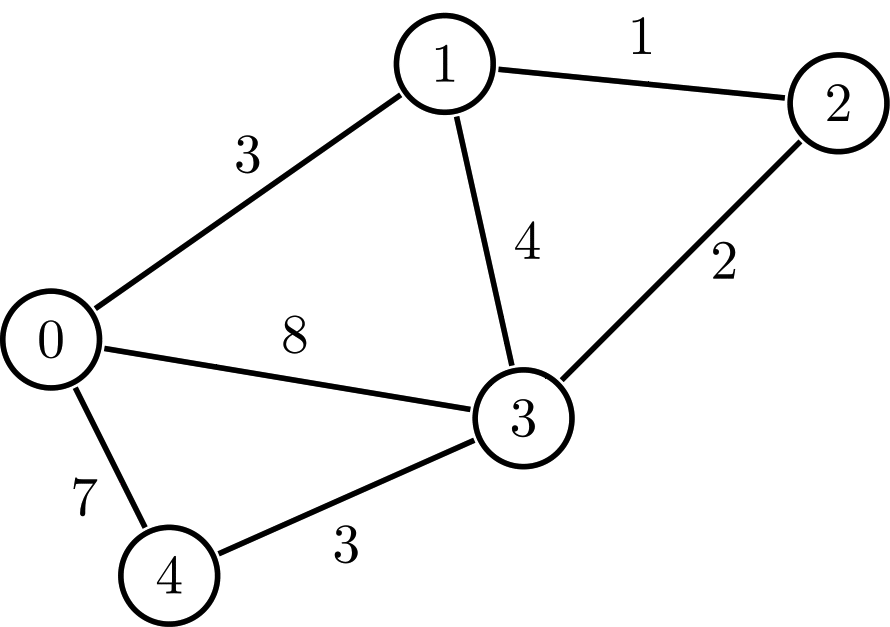
\includegraphics[width=\textwidth]{undirected-graph.png}
	\caption{Undirected graph with ordered edges and nodes}
	\label{fig:undirected-graph}
\end{marginfigure}
Note that definition \ref{def:graph} is general, and most of the times we are only concerned with \textit{simple graphs}, which have the following properties:
\begin{itemize}
	\item[$\diamond$] For any two nodes in the set $V$, there exists at most one edge between them.
	\item[$\diamond$] There are no self-loops, i.e for any $u \in V$, $(u, u) \notin E$.
	\item[$\diamond$] All edges of the graph are \textit{undirected}, i.e for $u, v \in V$, $(u, v) \in E \Leftrightarrow (v, u) \in E$.
\end{itemize}
\begin{definition}[Adjacency Matrix] \label{def:adjacency}
For a simple graph $G = (V, E)$, the adjacency matrix $\mathbf{A} \in \mathbb{R}^{|V| \times |V|}$ is a square matrix with $A_{uv} = 1$ if there is an edge from vertex $u$ to $v$, and $A_{uv} = 0$ otherwise.
\end{definition}
\marginnote{
\[\mathbf{A} = \begin{bmatrix}
	0 & 1 & 0 & 1 & 1 \\
	1 & 0 & 1 & 1 & 0 \\
	0 & 1 & 0 & 1 & 0 \\
	1 & 1 & 1 & 0 & 1 \\
	1 & 0 & 0 & 1 & 0
\end{bmatrix} \]
\begin{center}
The adjacency matrix for Fig \ref{fig:undirected-graph}.
\end{center}
}
Since we are dealing with simple graphs, some immediate consequences are that
\begin{itemize}
	\item[$\diamond$] $\mathbf{A}$ is symmetric, i.e $\mathbf{A}^T = \mathbf{A}$.
	\item[$\diamond$] $A_{uu} = 0 \; \forall \; u \in V$, i.e all diagonal elements are zero.
\end{itemize}
Notice that since we are defining the graph in terms of the matrix $\mathbf{A}$, we need to order the nodes prior to the representation (See Fig \ref{fig:undirected-graph}). An extension to definition \ref{def:adjacency} occurs when we allow the use of weighted edges, and in that case for $u, v \in V$, ${A}_{uv} \in [0, 1]$.

\subsection{Multi-relational Graphs}
We have noted three types of edges till now: undirected, directed and weighted. But for graphs, it is possible to have different types of edges. In such cases, we extend the notation to include relation type $\tau \in \mathcal{R}$ and write that $(u, \tau, v) \in E$ along with defining an adjacency matrix $\mathbf{A}_\tau$ for each type. The above class of graphs are called multi-relational, and are overall represented by an adjacency tensor $\mathcal{A} \in \mathbb{R}^{|V| \times |\mathcal{R}| \times |V|}$. Two major subsets of such graphs are:
\begin{enumerate}
	\item \textbf{Heterogeneous graphs:} We can partition the set of nodes into $k$ disjoint sets $V = \bigcup_{i=1}^k V_i$, and thus we have types imbued on nodes. 
	Usually in such graphs, we pose constraints on edges, for example they connect nodes of different types only (\textit{multipartite graphs}).
	\begin{marginfigure}
		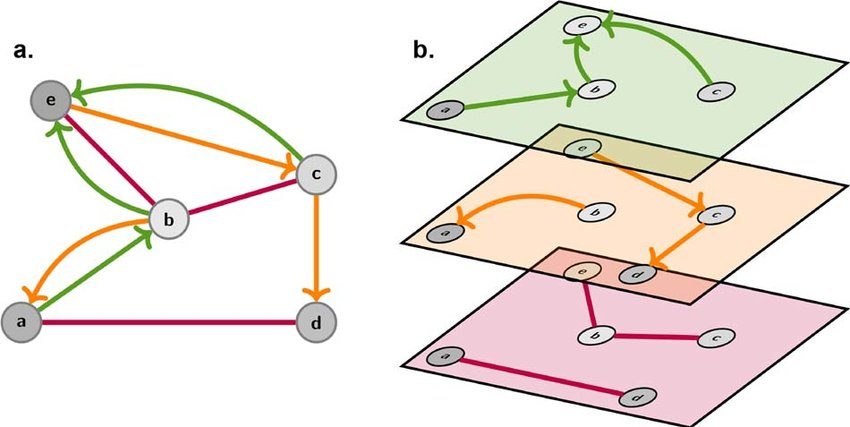
\includegraphics[width=\textwidth]{multi-relational-graph.png}
		\caption{Layered multiplex graph. Source: \cite{multiplexgraph}}
		\label{fig:multi-relational-graph}
	\end{marginfigure}
	\item \textbf{Multiplex graphs: }We can decompose such graphs into a set of layers (see Fig \ref{fig:multi-relational-graph}), and each node is in every layer with each layer possessing a unique relation. Edges will be present intra-layer and inter-layer.
\end{enumerate}

\subsection{Information representation}
Usually we have features representing graph-level features - may it be on nodes, edges or the entire graph itself. The most common one is node-level, and we associate an $m-$dimensional feature vector with each node, thus overall having a matrix $\mathbf{X} \in \mathbb{R}^{|V| \times m}$.

Now, let's go over some common graphical learning tasks.
\subsection{Node Classification}
	\begin{marginfigure}
	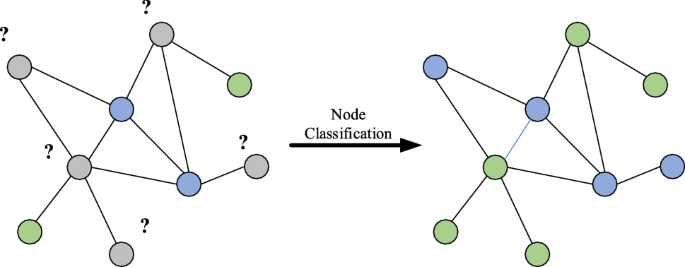
\includegraphics[width=\textwidth]{node-classification.png}
	\caption{Example of node classification. Source: \cite{node-classification-survey}}
	\label{fig:node-classification}
\end{marginfigure}
The goal of node classification is to predict a label $y_u$ associated with all nodes $u \in V$ when we have been only given the true labels of a subset of the nodes $V_{train} \subset V$. A few examples in literature of the task are:
\begin{enumerate}
	\item Interactome protein function classification: \cite{graphsage}
	\item Document classification based on citation graphs: \cite{gcn}
\end{enumerate}
Though it seems similar to supervised classification, there is a difficulty that the nodes in a graph are not \textit{i.i.d.} and thus we need to model dependencies between data points. This is exactly what node classification takes a benefit of through 
\begin{enumerate}
	\item \textbf{Homophily} \cite{homophily}: Tendency of nodes to share attributes with their neighbors
	\item \textbf{Structural Equivalence} \cite{structural-equivalence}: Idea that nodes with similar local neighborhood structures will have similar labels
	\item \textbf{Heterophily}: Presumption that nodes will be preferentially connected to differently-labeled nodes
\end{enumerate}
Note that, the only part of the network we don't access is the labels of the test nodes. We still have access to the structural information, and thus our task is \textbf{semi-supervised}.
\subsection{Link Prediction}
This task is related to the inference of edges between nodes in a graph. Given a set of nodes $V$ and an incomplete set of edges $E_{train} \subset E$, we want to infer the set $E \setminus E_{train}$. A few examples in literature of the task are:
\begin{marginfigure}
	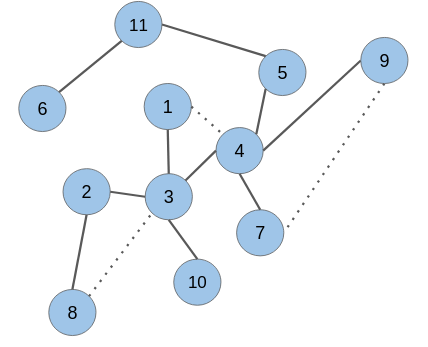
\includegraphics[width=\textwidth]{link-prediction.png}
	\caption{Example of node classification. Source: \href{https://www.analyticsvidhya.com/blog/2020/01/link-prediction-how-to-predict-your-future-connections-on-facebook/}{AnalyticsVidhya}}
	\label{fig:link-prediction}
\end{marginfigure}
\begin{enumerate}
	\item Content recommendation on social media: \cite{link-prediction-content}
	\item Modeling side-effects of drugs: \cite{link-prediction-side-effects}
\end{enumerate}
Although for simple graphs, we can have simple heuristics to give decent results \cite{link-prediction-survey-heuristic}, the task on multi-relational graphs is much more complex. \\
Much like node classification, the task boundary is smudged, and it falls under both supervised and unsupervised.
\subsection{Community Detection}
This task is the graphical analog of unsupervised learning. We want to infer latent community structures given only the input graph $G = (V, E)$. A few examples in literature of the task are:
\begin{enumerate}
	\item Uncovering functional modules in genetic interaction networks: \cite{community-detection-genetic}
	\item Fraud detection in financial transaction networks: \cite{community-detection-fraud}
\end{enumerate}
\subsection{Other popular graphical tasks}
\begin{itemize}
	\item[$\diamond$] \textbf{Graph Regression / Graph Classification}: In these tasks, we want to learn over graph data, and our dataset consists of multiple different graphs and we predict graph-wise. We can treat each graph as i.i.d and thus, the only challenge is to define useful features over graphs.
	\item[$\diamond$] \textbf{Graph Clustering} In this task, we learn an unsupervised measure of similarity between pairs of graphs.
\end{itemize}
\section{Traditional Approaches to Graph Learning}
\subsection{Node-level statistics}
Prior to advent of deep learning on graphs, a large part of machine learning on graphs was directed towards extraction of statistics/features based on heuristic functions and domain knowledge from graphs, and passing this information to a machine learning classifier. Now, we look over common node-level statistics.
\begin{definition}[Node degree]
The degree $d_u$ of a node $u \in V$ is the number of edges incident to a node, and in terms of $\mathbf{A}$ for a simple graph
\begin{equation} \label{eq:degree}
	d_u = \sum_{v \in V} A_{uv}
\end{equation}
If our graph is directed or weighted, we can have the notion of in-degree and out-degree by summing over rows or columns in Equation (\ref{eq:degree}).
\end{definition}
\marginnote{\textit{Perron-Frobenius Theorem}: A real square matrix with positive entries has a unique largest real eigenvalue, and the corresponding eigenvector can be chosen to have strictly positive components.}
\begin{definition}[Eigenvector Centrality]
The eigenvector centrality $e_u$ of a node $u \in V$ is defined by the recurrence relation
\begin{equation}
	e_u = \dfrac{1}{\lambda} \sum_{v\in V} A_{uv}e_v \; \forall \; u \in V
\end{equation}	
We can rewrite the above equation to notice that $\mathbf{A}\mathbf{e} = \lambda \mathbf{e}$ where $\mathbf{e}$ is the vector of node centralities.
\end{definition}
Note that, we want the centrality values to be positive, and by the \textbf{Perron-Frobenius Theorem}. 
In all, $\mathbf{e}$ is given by the eigenvector of the largest eigenvalue of $\mathbf{A}$. \marginnote{Note that the matrix $\mathbf{B}^{(n)}=\mathbf{A}^n$ has the elements such that $\mathbf{B}_{uv}^{(n)}$ denotes the number of $n-$length paths from $u \to v$.}
Now, since $\lambda$ is the leading eigenvalue, $e_u$ ranks the likelihood that a node is visited on a random-walk of infinite length on the graph as we can use power iteration method ($\mathbf{e^{(t)}} = \mathbf{A}\mathbf{e^{(t-1)}})$) to find $\mathbf{e}$. \\
By centrality, we can also measure how often a node lies on the shortest path between two nodes (\textit{betweeness centrality}), or average shortest path length between a node and all other nodes (\textit{closeness centrality}).
\begin{definition}[Clustering Coefficient]
The clustering coefficient \cite{small-world-dynamics} is given as
\begin{equation}
	c_u = \dfrac{|(v_1, v_2) \in E \; : \; v_1, v_2 \in \mathcal{N}(u)|}{{d_u \choose 2}}
\end{equation}	
It essentially measures the proportion of closed triangles in a node's local neighborhood.
\end{definition}
We can view clustering coefficient as the ratio between actual number of triangles and total possible number of triangles within a node's \textit{ego graph}: subgraph having the node, neighbors and all edges between nodes in its neighborhood.
\subsection{Graph Kernel Methods}
These methods are used for generating graph-level features for tasks such as graph classification.
\begin{definition}[Bag of Nodes]
Bag of nodes refers to aggregates of node-level statistics such as histograms based on clustering coefficients, and the use of such aggregates as graph-level features.
\end{definition}
Clearly bag of nodes misses global graph properties, and one way to improve it is to use iterative neighborhood aggregation.\\
    \begin{tcolorbox}[space to upper,
	skin=bicolor,
	colbacklower=black!75,
	collower=white,
	title={Weisfieler–Lehman Algorithm},
%	halign=center,
%	valign=center,
	nobeforeafter,
%	halign lower=flush right,
	bottom=0mm,
	height=6.4cm,
	width=4in
	]
	\begin{enumerate}
		\item Assign an initial label $\ell^{(0)}(v)$ to each node. A usual practice is to just assign the degree.
		\item Iteratively assign a new label by hashing the multiset of current labels within the neighborhood $$\ell^{(i)}(v) = \texttt{HASH}(\{\{\ell^{(i-1)}(u)\;\forall\;u \in \mathcal{N}(v)\}\})$$
		\item After running $K$ iterations of step-2, our label summarizes a $K$-hop neighborhood. Now use statistics of labels as features for the graphs.	
	\end{enumerate}
\end{tcolorbox}\\
\noindent The WL Kernel is computed by measuring the difference between the label sets of two graphs.
\begin{definition}[Graphlets]
Graphlets are small non-isomorphic induced subgraphs representing connected patterns in a network, and their frequency can be used to assess network structure.
\end{definition}
\begin{marginfigure}
	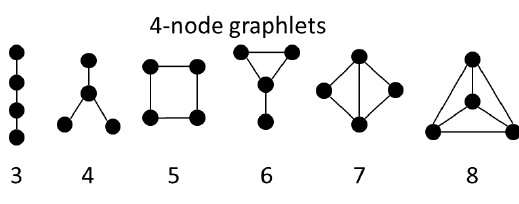
\includegraphics[width=\textwidth]{graphlets.png}
	\caption{Graphlets with 4 nodes}
	\label{fig:graphlets}
\end{marginfigure}
Graphlet kernels enumerate all graph structures of a possible size and count their occurrence in a graph. This is combinatorially difficult and an alternative is to use path-based methods which examine different kinds of paths in the graph. For example, the \textit{random-walk kernel} \cite{random-walk-kernel} involves running random walks all over the graph and then counting the occurrence of different degree sequences, while the \textit{shortest-path kernel} \cite{shortest-path-kernel} uses shortest paths between nodes instead of random-walks.

\subsection{Measures of Neighborhood Overlap}
Now we try to quantify the relation between nodes, which cannot be done using node-level or graph-level kernels. We denote $\mathbf{S} \in \mathbb{R}^{|V| \times |V|}$ as the similarity matrix summarizing the statistics. We commonly take the probability of an edge occurring proportional to the statistical measure, i.e $\mathbb{P}(A_{uv} = 1) \propto \mathbf{S}[u,v]$.
\begin{enumerate}
	\item \textit{Local overlap measures}
\begin{enumerate}
\item \textbf{Common Neighbors (CN)}: It is the simplest neighborhood overlap measure and counts the number of neighbors two nodes share.
\begin{equation}
	\mathbf{S}_{CN}[u, v] = |\mathcal{N}(u) \cap \mathcal{N}(v)|
\end{equation}	
We can extend the idea to local overlap measures defined over CN, denoted by the next three quantifiers.
\item \textbf{Sorensen index}: This normalizes the counts of common neighbours by the sum of node-degrees.
\begin{equation}
	\mathbf{S}_{Sorensen}[u, v] = \dfrac{2|\mathcal{N}(u) \cap \mathcal{N}(v)|}{d_u + d_v}
\end{equation}
\item \textbf{Salton index}: This normalizes using the product of degrees.
\begin{equation}
	\mathbf{S}_{Salton}[u, v] = \dfrac{2|\mathcal{N}(u) \cap \mathcal{N}(v)|}{\sqrt{d_ud_v}}
\end{equation}
\item \textbf{Jaccard index}: This is an IOU measure.
\begin{equation}
	\mathbf{S}_{Jaccard}[u, v] = \dfrac{|\mathcal{N}(u) \cap \mathcal{N}(v)|}{|\mathcal{N}(u) \cup \mathcal{N}(v)|}
\end{equation}
\item \textbf{Resource Allocation (RA)}: It places importance on the common neighbors by summing the inverse degrees, i.e
\begin{equation}
	\mathbf{S}_{RA}[u, v] = \sum_{w \in \mathcal{N}(u) \cap \mathcal{N}(v)} \dfrac{1}{d_w}
\end{equation}
\item \textbf{Adamic-Adar (AA)}: It is similar to RA, just utilizes inverse log of the degrees, i.e
\begin{equation}
	\mathbf{S}_{AA}[u, v] = \sum_{w \in \mathcal{N}(u) \cap \mathcal{N}(v)} \dfrac{1}{\log d_w}
\end{equation}
Both these measures infer that common neighbors with low degrees are more informative.
\end{enumerate}
\item \textit{Global overlap measures}
\begin{enumerate}
	\item \textbf{Katz Index}: We take a discounted count of number of paths of all lengths between a pair of nodes, i.e
	\begin{equation}
		\mathbf{S}_{Katz}[u, v] = \sum_{i=1}^\infty \beta^i A_{uv}^i = \Big((\mathbf{I} - \beta \mathbf{A})^{-1} - \mathbf{I}\Big)[u,v]
	\end{equation}
	Here $\beta \in \mathbb{R}^+$ is our discount, and a small $\beta < 1$ down-weights the importance of long-paths.
\end{enumerate}
\end{enumerate}
\section{Learning Node Embeddings}
Following \cite{node-emb-latent-space}, we project nodes into a latent space and the geometric relations in that space correspond to those in the original graph.
\begin{marginfigure}
	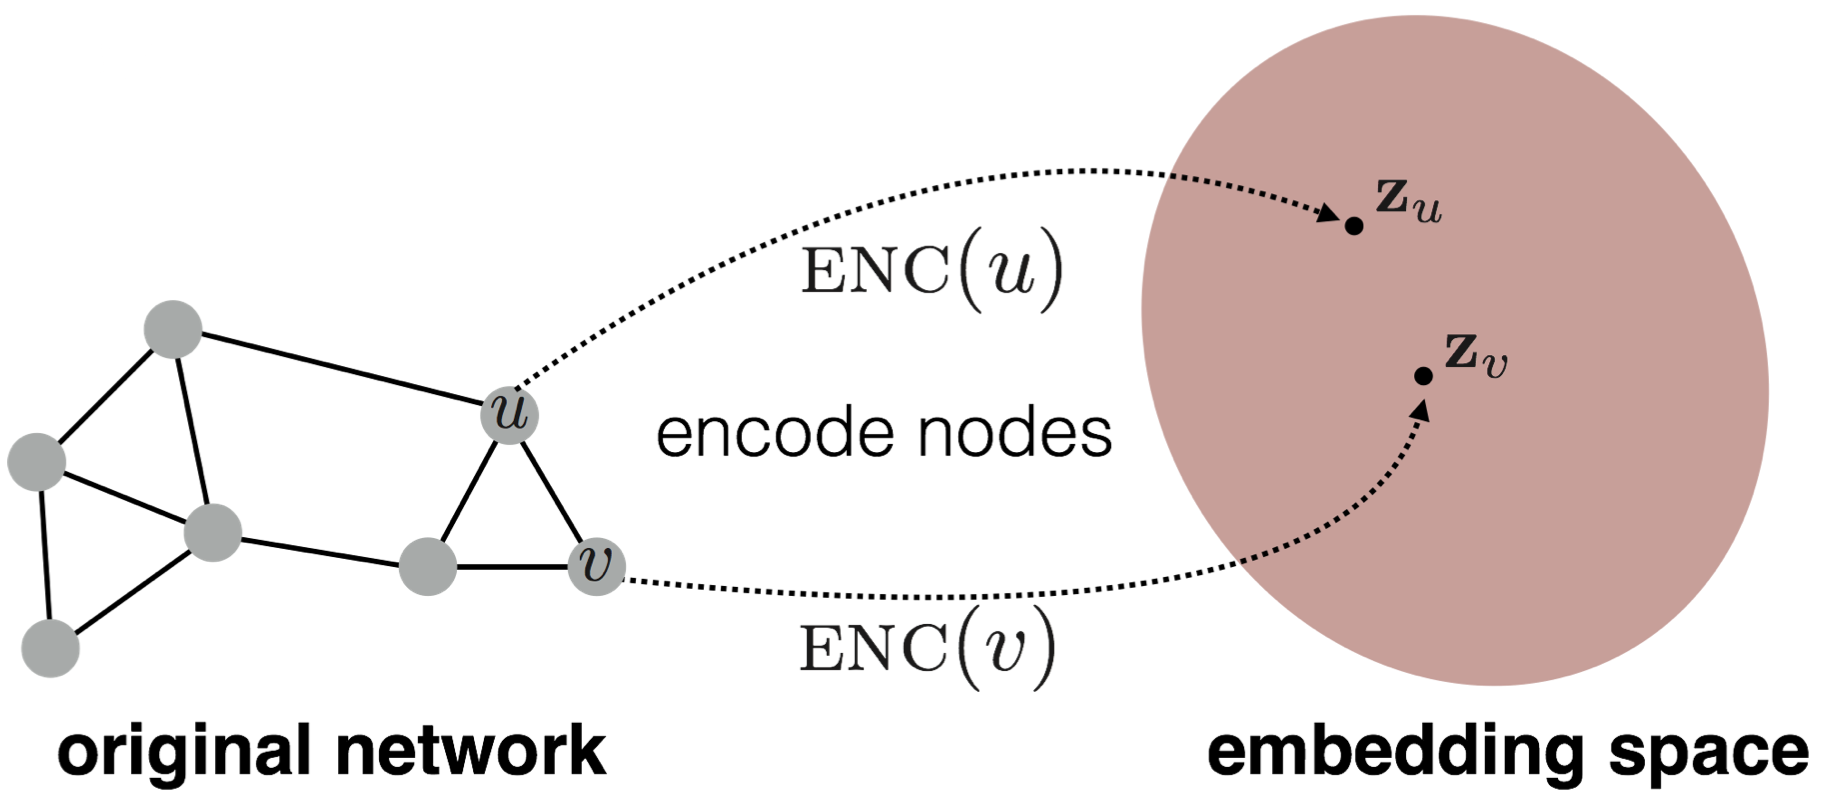
\includegraphics[width=\textwidth]{node-embeddings.png}
	\caption{Node Representation Learning Source: \href{https://snap-stanford.github.io/cs224w-notes/machine-learning-with-networks/node-representation-learning}{Stanford}}
	\label{fig:node-embedding}
\end{marginfigure}
\subsection{Encoder-Decoder Model}
The task is essentially to \textit{encode} each node into a low-dimensional vector, and finally \textit{decode} the embedding and use it to reconstruct information \cite{representation-learning-methods}.
\begin{definition}[Encoder]
The encoder is a function \texttt{ENC}$:V \to \mathbb{R}^d$ which maps nodes $v \in V$ to vector embeddings $\mathbf{z}_v \in \mathbb{R}^d$.. Commonly the approach is a shallow embedding one, and thus the encoder function is an embedding lookup on the node ID, i.e \texttt{ENC}$(v) = \mathbf{Z}[v]$ where $\mathbf{Z} \in \mathbb{R}^{|V| \times d}$ is the embedding matrix.
\end{definition}
\begin{definition}[Decoder]
The decoder reconstructs certain graph statistics from node embeddings generated by the encoder. It is common to use pairwise decoders, i.e \texttt{DEC}$:\mathbb{R}^d \times \mathbb{R}^d \to \mathbb{R}^+$ and they are similarity measures.
\end{definition}
The goal is to minimize reconstruction loss, i.e 
\begin{equation}\label{eq:recon-loss}
\texttt{DEC}(\texttt{ENC}(u), \texttt{ENC}(v)) = \texttt{DEC}(\mathbf{z}_u, \mathbf{z}_v) \approx \mathbf{S}[u, v]
\end{equation}
\marginnote{
	Mean Squared Error loss:
	\begin{equation*}
		MSE(y, \tilde{y}) = \dfrac{1}{n}\sum_{i=1}^n (y_i - \tilde{y}_i)^2
	\end{equation*}
	Cross Entropy loss:
	\begin{equation*}
		CE(y, \tilde{y}) = -\dfrac{1}{n}\sum_{i=1}^n y_i \log(\tilde{y}_i)
	\end{equation*}
}
To achieve the goal above, we minimize an empirical reconstruction loss function
\begin{equation}
\mathcal{L} = \sum_{(u, v) \in \mathcal{D}} \ell(\texttt{DEC}(\mathbf{z}_u, \mathbf{z}_v), \mathbf{S}[u,v])
\end{equation}
\noindent where $\mathcal{D}$ is a subset of node pairs, and $\ell$ is a loss function such as cross-entropy or mean-squared error loss. We look at some common shallow embedding algorithms:
\begin{enumerate}
\item \textbf{Factorization based Encoder-Decoder}\\
The loss function for such approaches can be minimized using factorization algorithms such as SVD.
\begin{enumerate}
\item \textbf{Laplacian Eigenmaps} \cite{laplacian-eigenmaps}: 
	\marginnote{If we construct $\mathbf{S}$ to satisfy properties of $\mathbf{L}$, and $\mathbf{z}_u$ are $d$-dimensional, then the optimal solution for minimizing the loss is given by the $d$ smallest eigenvectors of $\mathbf{L}$ excluding the smallest one, i.e $\mathbf{1}$}
It is an old but influential approach built upon spectral clustering. The decoder is 
\begin{equation}
	\texttt{DEC}(\mathbf{z}_u, \mathbf{z}_v) = ||\mathbf{z}_u - \mathbf{z}_v||_2^2
\end{equation}
and the loss function is
 \begin{equation}
\mathcal{L} = \sum_{(u,v) \in \mathcal{D}} \texttt{DEC}(\mathbf{z}_u, \mathbf{z}_v)\mathbf{S}[u,v]
\end{equation}
\item \textbf{Inner-product methods}: The decoder in these is 
\begin{equation}
\texttt{DEC}(\mathbf{z}_u, \mathbf{z}_v) = \mathbf{z}_u^T\mathbf{z}_v
\end{equation}
and the loss function is
\begin{equation}
\mathcal{L} = \sum_{(u,v) \in \mathcal{D}} ||\texttt{DEC}(\mathbf{z}_u, \mathbf{z}_v) - \mathbf{S}[u,v]||_2^2
\end{equation}

\begin{enumerate}
	\item \textit{Graph Factorization} \cite{graph-factorization}: It uses $\mathbf{S} \triangleq \mathbf{A}$.
	\item \textit{GraRep} \cite{grarep}: It defines $\mathbf{S}$ based on powers of $\mathbf{A}$.
	\item \textit{HOPE} \cite{hope}: It defines $\mathbf{S}$ based on neighborhood overlap measures.
\end{enumerate}
\end{enumerate}
\item \textbf{Random Walk Embeddings} \\
The notion in such embeddings are that two nodes have similar embeddings if they tend to co-occur on short random walks over the graph. We learn embeddings to get
\begin{equation} \label{eq:random-walk-decoder}
\texttt{DEC}(\mathbf{z}_u, \mathbf{z}_v) \triangleq \dfrac{e^{\mathbf{z}_u^T \mathbf{z}_v}}{\sum_{w \in V} e^{\mathbf{z}_u^T \mathbf{z}_w}} \approx p_{G, T}(v|u)
\end{equation}
\marginnote{The notation $\Iintv{x,y}$ denotes the integer interval spanning from $x$ to $y$, i.e $\{x, \cdots y\}$}
where $p_{G,T}(v|u)$ is the probability of reaching node $v$ starting at $u$ on a $T$-length random walk ($T \in \Iintv{2, 10}$). Clearly the decoder is learning an asymmetric stochastic measure. To train the embeddings, the loss function employed is
\begin{equation}
\mathcal{L} = \sum_{(u,v) \in \mathcal{D}} -\log(\texttt{DEC}(\mathbf{z}_u, \mathbf{z}_v))
\end{equation}
	\marginnote{It has been shown in \cite{network-embedding-matrix} that if we define 
	\begin{equation*}
		\mathbf{S}_{DW} = \log\bigg(\dfrac{\sum_{w \in V}d_w}{T} \Big(\sum_{t=1}^T\mathbf{P}^t\Big)\mathbf{D}^{-1}\bigg) - \log (b)
	\end{equation*}
	then, the embeddings $\mathbf{Z}$ by DeepWalk satisfy $\mathbf{Z}^T \mathbf{Z} \approx \mathbf{S}_{DW}$. What is interesting to note that is we can eigendecompose the interior of above equation, and note that DeepWalk is closely related to $\mathbf{L}_{sym}$ and hence spectral clustering, but differ by the fact that influence of eigenvalues is controlled by DeepWalk through $T$.
}
But the issue here is that evaluating the loss function has time complexity $\mathcal{O}(|V||\mathcal{D}|) \sim \mathcal{O}(|V|^2)$.
\begin{enumerate}
	\item \textbf{DeepWalk} \cite{deepwalk}: 
	It employs uniformly random walks to define $p_{G,T}(v|u)$ and employs hierarchical softmax \cite{hierarchical-softmax} to approximate Equation (\ref{eq:random-walk-decoder})
	\item \textbf{node2vec} \cite{node2vec}: It introduces hyperparameters to allow random walk probabilities to interpolate between walks more akin to BFS or DFS. It uses noise contrastive estimation along with negative sampling to rewrite $\mathcal{L}$ as
	\begin{equation}
	\mathcal{L} = \sum_{(u,v)\in\mathcal{D}} -\log(\sigma(\mathbf{z}_u^T\mathbf{z}_v)) - \gamma \mathbb{E}_{v_n \sim P_n(V)}[\log(-\sigma(\mathbf{z}_u^T \mathbf{z_{v_n}}))]
	\end{equation}
	with $\gamma > 0$ and $P_n(V)$ being the uniform distribution. Monte Carlo Sampling is used to calculate the expectation.
	\item \textbf{LINE} \cite{line}: It proposes a first objective
	\begin{equation}
		\texttt{DEC}(\mathbf{z}_u, \mathbf{z}_v) = \sigma(\mathbf{z}_u^T\mathbf{z}_v)
	\end{equation}
\marginnote{
\textbf{KL-Divergence}
\begin{equation*}
	D_{KL}(p \parallel q) = \sum_{i=1}^n p(x_i) \log\bigg(\dfrac{p(x_i)}{q(x_i)}\bigg)
\end{equation*}
}
and $\mathbf{S}[u,v] = A_{uv}$. Along with that, a second objective is the decoder same as DeepWalk, but trained using KL-Divergence to encode 2-hop information (i.e $\mathbf{A}^2$), and it explicitly reconstructs first and second-order neighborhood information.
\end{enumerate}
\end{enumerate}
\subsection{Drawbacks of Shallow Embeddings}
\begin{itemize}
	\item[$\diamond$] Lack of parameter sharing between nodes is a hinder to statistic and computational efficiency. We want embeddings to be independent of $|V|$.
	\item[$\diamond$] They do not leverage node features in \texttt{ENC}.
	\item[$\diamond$] They are transductive, and thus it is difficult to generate embeddings for newer nodes and cannot be used in inductive applications which involve generalization.
\end{itemize}
\marginnote{\textbf{Knowledge Graphs}: They are multi-relational graphs $G = (V,E)$ with edges defined as tuples $e = (u, \tau, v)$ indicating the presence of a relation $\tau \in \mathcal{R}$ between two nodes. The task of knowledge graph completion is generally to predict the missing edges in the graph.}
\subsection{Reconstruction of Multi-Relational Data}
Multi-relational graphs add a relation type, and to address that, we make the decoder multi-relational, i.e $\texttt{DEC}: \mathbb{R}^d \times \mathcal{R} \times \mathbb{R}^d \to \mathbb{R}^+$.
\textbf{RESCAL} \cite{rescal} defines the multi-relational decoder as $\texttt{DEC}(u, \tau, v) = \mathbf{z}_u^T \mathbf{R}_\tau \mathbf{z}_v$, where $\mathbf{R}_\tau$ is a learnable matrix for relation $\tau \in \mathcal{R}$, and we can learn $\mathbf{Z}$ and $\mathbf{R}_\tau$ using a simple reconstruction loss 
\begin{equation} \label{eq:mr-recon-loss}
\mathcal{L} = \sum_{u\in V} \sum_{v\in V} \sum_{\tau \in \mathcal{R}} ||\mathbf{z}_u^T \mathbf{R}_\tau \mathbf{z}_v - \mathcal{A}_{u\tau v}||^2]
\end{equation}
As seen above, it is a common practice to define the similarity measure based on the adjacency tensor, and thus we are trying to reconstruct immediate neighbors from the embeddings. \\
\begin{enumerate}
\item \textbf{Loss Functions}: The loss defined in Equation (\ref{eq:mr-recon-loss}) requires $\mathcal{O}(|V|^2|\mathcal{R}|)$ time complexity, and is extremely expensive. Since it is realistically seen that multi-relational graphs are sparse, we would want a loss function of the order $\mathcal{O}(|E|)$. Also, since our target is to decode the adjacency tensor, which has binary values, we can't use the simple MSE loss.
\begin{enumerate}
	\item \textbf{Cross-Entropy with Negative Sampling}: Defining $\sigma$ as the sigmoid function, $P_{n,u}(V)$ as the negative sampling distribution, and $\gamma > 0$, we write
	\begin{equation}
	\begin{split}
	\mathcal{L} = \sum_{(u, \tau, v) \in E}\bigg(& -\log(\sigma(\texttt{DEC}(\mathbf{z}_u, \tau, \mathbf{z}_v))) \\&- \gamma \mathbb{E}_{v_n \sim P_{n, u}(V)}[\log(\sigma(-\texttt{DEC}(\mathbf{z}_u, \tau, \mathbf{z}_{v_n})))] \bigg)
	\end{split}
	\end{equation}
If we calculate the expectation using Monte Carlo Sampling, we can write by sampling over a small subet $\mathcal{P}_{n,u} \subset P_{n,u}(V)$
\begin{equation}
\mathcal{L} = -\sum_{(u, \tau, v) \in E}\log(\sigma(\texttt{DEC}(\mathbf{z}_u, \tau, \mathbf{z}_v)))	- \sum_{v_n \in \mathcal{P}_{n, u}}\log(\sigma(-\texttt{DEC}(\mathbf{z}_u, \tau, \mathbf{z}_{v_n})))
\end{equation}
	\item \textbf{Max-Margin Loss}: Also called the \textit{hinge loss}, we set a margin $\Delta$ and use \textit{contrastive estimation} (but with direct comparison of output of the decoders) to write the loss function as
	\begin{equation}
		\mathcal{L} = \sum_{(u, \tau, v) \in E} \sum_{v_n \in \mathcal{P}_{n, u}} \max(0, -\texttt{DEC}(\mathbf{z}_u, \tau, \mathbf{z}_v) + \texttt{DEC}(\mathbf{z}_u, \tau, \mathbf{z}_{v_n}) + \Delta)
	\end{equation}
\end{enumerate}
\item \textbf{Decoders}:
\begin{enumerate}
	\item \textbf{RESCAL}: In the RESCAL decoder, a trainable matrix $\mathbf{R}_\tau \in \mathbb{R}^{d \times d}$ is associated with each relation
	\begin{equation}
		\texttt{DEC}(\mathbf{z}_u, \tau, \mathbf{z}_v) = \mathbf{z}_u^T \mathbf{R}_\tau \mathbf{z}_v
	\end{equation}
	 This gives rise to $\mathcal{O}(d^2)$ number of parameters for each relation, and that has high computational cost. Recent decoders aim to get $\mathcal{O}(d)$ number of parameters.
	 \item \textbf{Translational Decoders}: Such decoders represent relations as translations in embedding space. 
	 \begin{enumerate}
	 	\item \textbf{TransE} \cite{transe}: Using a $d$-dimensional embedding, the decoder is
	 	\begin{equation}
	 		\texttt{DEC}(\mathbf{z}_u, \tau, \mathbf{z}_v) = -||\mathbf{z}_u + \mathbf{r}_\tau - \mathbf{z}_v||
	 	\end{equation}
 	It is a simple decoder, and the likelihood of an edge is proportional to the distance translated according to the relation.
 	\item \textbf{TransX}: These are a class of models built upon the TransE model, and have the general form
 	\begin{equation}
 		\texttt{DEC}(\mathbf{z}_u, \tau, \mathbf{z}_v) = -||g_{1, \tau}(\mathbf{z}_u) + \mathbf{r}_\tau - g_{2,\tau}(\mathbf{z}_v)||
 	\end{equation}
 where $g_{i,\tau}$ are trainable transformations. \cite{transh} proposed the TransH model which projects the entity embeddings onto a learnable relation-specific hyperplane defined by the normal vector $\mathbf{w}_r$ and then translating it.
 \begin{equation}
 	\texttt{DEC}(\mathbf{z}_u, \tau, \mathbf{z}_v) = -||(\mathbf{z}_u - \mathbf{w}_r^T \mathbf{z}_u \mathbf{w}_r) + \mathbf{r}_\tau - (\mathbf{z}_v - \mathbf{w}_r^T \mathbf{z}_v \mathbf{w}_r)||
 \end{equation}
	 \end{enumerate}
 \item \textbf{DistMult} \cite{distmult}: This generalizes the dot-product decoder from simple graphs, thus
 \begin{equation}
 	\texttt{DEC}(\mathbf{z}_u, \tau, \mathbf{z}_v) = \langle \mathbf{z}_u, \mathbf{r}_\tau, \mathbf{z}_v \rangle = \sum_{i=1}^d \mathbf{z}_u[i] \times \mathbf{r}_\tau[i] \times \mathbf{z}_v[i]
 \end{equation}
This has a restriction, that it can only be used for symmetric relations, but majority of the relation are assymetric.
\item \textbf{ComplEx} \cite{complex}: This extends the above idea and uses complex-valued embeddings, to bring in asymmetry, i.e $\mathbf{z}_u, \mathbf{r}_\tau, \mathbf{z}_v \in \mathbb{C}^d$.
 \begin{equation}
	\texttt{DEC}(\mathbf{z}_u, \tau, \mathbf{z}_v) = \Re\langle \mathbf{z}_u, \mathbf{r}_\tau, \bar{\mathbf{z}}_v \rangle =\Re\bigg( \sum_{i=1}^d \mathbf{z}_u[i] \times \mathbf{r}_\tau[i] \times \bar{\mathbf{z}}_v[i]\bigg)
\end{equation}
\item \textbf{RotatE} \cite{rotate}: This is again a complex-valued decoder, with the constraint that $|\mathbf{r}_\tau[i]| = 1 \implies \mathbf{r}_\tau[i] =e^{\iota \theta_{r, i}}$. This brings in rotations in the complex plane, and 
\begin{equation}
	\texttt{DEC}(\mathbf{z}_u, \tau, \mathbf{z}_v) = - || \mathbf{z}_u \circ \mathbf{r}_\tau - \mathbf{z}_v||
\end{equation}
\end{enumerate}
\end{enumerate}
\subsection{Representation Abilities of Multi-Relational Decoders}
We characterize the representation abilities of the multi-relational decoders in three ways:
\marginnote{Symmetric relations mean that \[ (u, \tau, v) \in E \leftrightarrow (v, \tau, u) \in E\]
Anti-symmetric relations mean that \[ (u, \tau, v) \in E \rightarrow (v, \tau, u) \notin E\]}
\begin{itemize}
	\item[$\diamond$] \textbf{Symmetry}: Can different decoders model both symmetric and anti-symmetric relations? DistMult can only model symmetric, while TransE can only model anti-symmetric, while all others are seen to model both.
	\marginnote{Inversion means that \[ (u, \tau_1, v) \in E\leftrightarrow (v, \tau_2, u) \in E\]}
	\item[$\diamond$] \textbf{Inversion}: Most decoders can model inversion, though TransX and DistMult fail in this respect.
	\marginnote{Compositionality means that \[(u, \tau_1, y) \in E \land (y, \tau_2, v) \in E \rightarrow (u, \tau_3, v) \in E\]}
	\item[$\diamond$] \textbf{Compositionality}: It is seen that in RESCAL, defining $\mathbf{R}_{\tau_3} = \mathbf{R}_{\tau_1}\mathbf{R}_{\tau_2}$ and in TransE defining $\mathbf{r}_{\tau_3} = \mathbf{r}_{\tau_1} + \mathbf{r}_{\tau_2}$ allows modeling of compositionality. RotateE also models it, while the rest three decoders we saw fail to do so.
\end{itemize}


\nocite{*}
\footnotesize
\bibliographystyle{apalike}
\bibliography{notes1/reference}

\end{document}
